\section{Supplement}
%===================================================================================================
\subsection{Source Data}\label{app.data}
Table~\ref{tab:data} gives the RDS-adjusted data from \cite{Baral2014}.
\begin{table}[h]
  \centering
  \caption{RDS-adjusted proportions for variables of interest}
  \label{tab:data}
  \begin{tabular}{llrc}
  \toprule
  Variable           & Stratum & Mean & (\ci) \\
  \midrule
  Years selling sex
    & 0--2    & 38.3 & (27.5,~49.1) \\
    & 3--5    & 32.1 & (23.6,~40.7) \\
    & 6--10   & 20.2 & (13.2,~27.1) \\
    & 11+     &  9.4 & (04.4,~14.4) \\[1ex]
  New clients\tn{a}
    & 0--1    & 16.4 & (09.8,~23.0) \\
    & 2       & 43.4 & (33.3,~53.5) \\
    & 3       & 15.2 & (09.6,~20.9) \\
    & 4       & 13.1 & (07.0,~19.2) \\
    & 5       & 11.8 & (06.0,~17.6) \\[1ex]
  Regular clients\tn{a}
    & 0--1    & 10.0 & (01.9,~18.1) \\
    & 2       &  8.5 & (03.2,~13.8) \\
    & 3       & 15.9 & (09.8,~21.9) \\
    & 4       & 10.0 & (04.5,~15.6) \\
    & 5       &  8.1 & (03.8,~12.3) \\
    & 6       & 10.7 & (05.8,~15.5) \\
    & 7+      & 36.9 & (26.4,~47.3) \\[1ex]
  Non-paying partners\tn{a} 
    & 0       & 12.5 & (04.8,~20.1) \\
    & 1       & 50.8 & (42.9,~58.7) \\
    & 2       & 23.6 & (16.8,~30.3) \\
    & 3+      & 13.2 & (07.2,~19.1) \\
  \bottomrule
\end{tabular}
\floatfoot{\vskip1ex\centering%
  \tnt[a]{Number reported in the past 30 days.}
  Data from \cite{Baral2014}.}

\end{table}
%===================================================================================================
\subsection{Code}\label{app.code}
All analysis code is available online at: \hreftt{github.com/mishra-lab/duration-bias}.\\
We fit the generative models using rjags: \hreftt{cran.r-project.org/package=rjags},\\
with 1000 adaptive iterations and 100,000 sampling iterations.
%===================================================================================================
\subsection{Beta Approximation of the Binomial Distribution}\label{app.bab}
The distributions of RDS-adjusted variables in \cite{Baral2014} were reported as
adjusted proportions (mean, \ci) for different variable value strata.
For each proportion, we defined a beta approximation of the binomial (BAB) distribution:
\begin{align}\label{eq:bab}
  \distr{P}{\rho} &=
    \frac{\Gamma(\alpha+\beta)}{\Gamma(\alpha)\,\Gamma(\beta)}\,
    \rho^{\alpha-1}{(1 - \rho)}^{\beta-1} \\
    &\approx {N \choose n} \, \rho^{n}{(1 - \rho)}^{N - n} \nonumber
\end{align}
with $\alpha = N\,\rho$ and $\beta = N\,(1-\rho)$.
We fixed $\rho$ as the adjusted point estimate,
and estimated $N$ by minimizing the sum of squared differences between
the 95\% quantiles of \eqref{eq:bab} given $N$ and the reported \ci for the adjusted proportion.
%===================================================================================================
\subsection{Risk Group Duration}\label{app.yss}
%---------------------------------------------------------------------------------------------------
\paragraph{Fitting to RDS-Adjusted Proportions}
Figure~\ref{fig:yss.fit} illustrates
the observed \vs inferred proportions of women reporting
different durations selling sex,
following each stage of adjustment outlined in \sref{meth.yss}.
\begin{figure}[h]
  \centering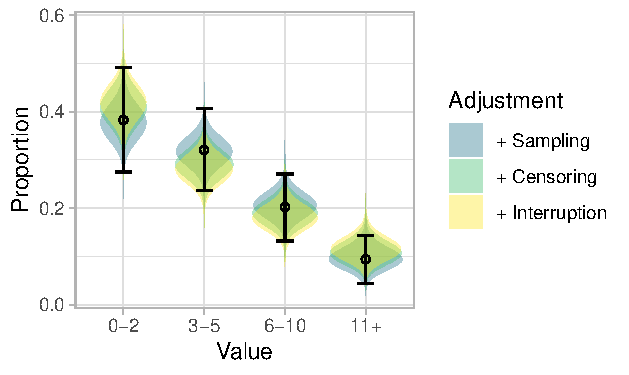
\includegraphics[scale=.8]{yss.fit}
  \caption{Proportions of women reporting different durations selling sex:
    observed (points and ranges) \vs inferred posterior (coloured regions)
    after 3 stages of adjustment}
  \label{fig:yss.fit}
\end{figure}
%---------------------------------------------------------------------------------------------------
\paragraph{Numeric Summary}
Table~\ref{tab:yss.adj} summarizes the estimated exponential distribution means (\ci)
for years selling sex following each stage of adjustment outlined in \sref{meth.yss}.
\begin{table}[h]
  \centering
  \caption{Estimated mean durations selling sex (years) following each stage of adjustment}
  \label{tab:yss.adj}
  \begin{tabular}{lrc}
  \toprule
  Adjustment     & Mean & (\ci) \\
  \midrule
  Median         & 4.00 & --- \\
  Mean           & 5.77 & --- \\
  + Sampling     & 4.35 & (3.27,~\w5.72) \\
  + Censoring    & 9.40 & (6.60,~13.22) \\
  + Interruption & 4.06 & (2.29,~\w6.34) \\
  \bottomrule
\end{tabular}

\end{table}
%===================================================================================================
\subsection{Rate of Partnership Change}\label{app.parts}
%---------------------------------------------------------------------------------------------------
\paragraph{Fitting to RDS-Adjusted Proportions}
Figure~\ref{fig:parts.fit} illustrates
the observed \vs inferred proportions of women reporting
different numbers of partners in the past 30 days,
under each partnership duration assumption outlined in \sref{meth.parts}.
\begin{figure}[h]
  \centering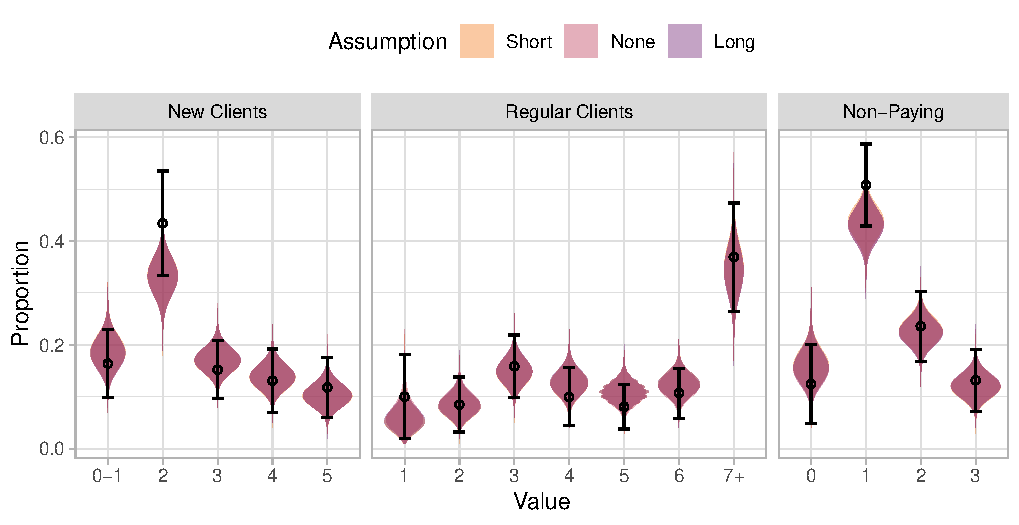
\includegraphics[scale=.8]{parts.fit}
  \caption{Proportions of women reporting different numbers of partner in the past 30 days:
    observed (points and ranges) \vs inferred posterior (coloured regions)
    under different partnership duration assumptions}
  \label{fig:parts.fit}
\end{figure}
%---------------------------------------------------------------------------------------------------
\paragraph{Numeric Summary}
Table~\ref{tab:parts.fsw} summarizes the means (\ci) for
rates of partnership change and numbers of current partners
estimated under each partnership duration assumption outlined in \sref{meth.parts}.
\begin{table}[h]
  \centering
  \caption{Biased \vs unbiased estimates of
    rates of partnership change and numbers of current partners
    for three partnership types}
  \label{tab:parts.fsw}
  \begin{tabular}{llrcrc}
  \toprule
   & & \multicolumn{2}{c}{Rate $Q$\tn{a}} &
       \multicolumn{2}{c}{Number $K$} \\
  \cmidrule(rl){3-4}\cmidrule(rl){5-6}
  Partnership Type & Bias\tn{b} & Mean & (\ci) & Mean & (\ci) \\
  \midrule
  New Clients     & Biased   & 2.82 & (2.33,~3.35) & 2.84 & (2.36,~3.37) \\
                  & Unbiased & 2.75 & (2.29,~3.31) & 0.09 & (0.08,~0.11) \\
  Regular Clients & Biased   & 5.38 & (4.60,~6.20) & 5.33 & (4.57,~6.19) \\
                  & Unbiased & 1.07 & (0.90,~1.25) & 4.28 & (3.62,~5.02) \\
  Non-Paying      & Biased   & 1.49 & (1.17,~1.86) & 1.54 & (1.20,~1.95) \\
                  & Unbiased & 0.04 & (0.03,~0.05) & 1.51 & (1.18,~1.88) \\
  \bottomrule
\end{tabular}
\floatfoot{\vskip1ex\centering
  \tnt[a]{Rates are per-month};
  \tnt[b]{biased $Q$ assume short partnerships as in \eqref{eq:bQ};
          biased $K$ assume long partnerships as in \eqref{eq:bK}}.}

\end{table}
\printbibliography
